\documentclass[aspectratio=169,professionalfonts]{beamer}

\usepackage[T1]{fontenc}
\usepackage{textcomp}
\usepackage{lmodern}
\usepackage{graphicx}
\usepackage{tikz}
\usetikzlibrary{arrows.meta}

\definecolor{Midnight}{HTML}{071827}
\definecolor{Panel}{HTML}{102D43}
\definecolor{Cyan}{HTML}{35D6E6}
\definecolor{Teal}{HTML}{18B7B5}
\definecolor{Ink}{HTML}{F2F7FA}
\definecolor{Muted}{HTML}{A9C3D1}
\definecolor{Rule}{HTML}{34576A}

\setbeamercolor{normal text}{fg=Ink,bg=Midnight}
\setbeamercolor{background canvas}{bg=Midnight}
\setbeamertemplate{navigation symbols}{}
\setbeamertemplate{headline}{}
\setbeamertemplate{footline}{}
\setbeamertemplate{frametitle}{}
\setlength{\parindent}{0pt}
\hypersetup{
  pdftitle={ParallaX | SPHEREx blink comparator},
  pdfauthor={The ParallaX team},
  pdfsubject={2026 NASA Space Apps Challenge: Planet X and SPHEREx},
  unicode=true
}
\graphicspath{{assets/}}

\newcommand{\CoverSource}{https://www.jpl.nasa.gov/images/pia26600-spherexs-first-all-sky-map/}
\newcommand{\VelaSource}{https://science.nasa.gov/open-science/spherex-universe-map/}
\newcommand{\Archive}{https://irsa.ipac.caltech.edu/Missions/spherex.html}
\newcommand{\BYWSource}{https://science.nasa.gov/get-involved/citizen-science/nasa-volunteers-double-known-population-of-brown-dwarfs/}
\newcommand{\Link}[2]{\href{#1}{\textcolor{Cyan}{#2}}}
\newcommand{\DeckTitle}[1]{{\fontsize{22}{24}\selectfont\bfseries #1}}
\newcommand{\Display}[1]{{\fontsize{27}{29}\selectfont\bfseries #1}}
\newcommand{\Subhead}[1]{{\fontsize{11.2}{13.2}\selectfont\bfseries #1}}
\newcommand{\ItemHead}[1]{{\fontsize{10.4}{12}\selectfont\bfseries #1}}
\newcommand{\Body}[1]{{\fontsize{10.4}{13.1}\selectfont #1}}
\newcommand{\SmallBody}[1]{{\fontsize{9.1}{11.5}\selectfont #1}}
\newcommand{\Note}[1]{{\fontsize{8.2}{10}\selectfont #1}}
\newcommand{\Caption}[1]{{\color{Muted}\fontsize{7.4}{9.1}\selectfont #1}}
\newcommand{\Label}[1]{{\color{Cyan}\fontsize{7.8}{9.3}\selectfont\bfseries #1}}
\newcommand{\Copy}[2]{\parbox[t]{#1mm}{\raggedright\setlength{\baselineskip}{11.5pt}#2\par}}
\newcommand{\um}{\,\textmu m}
\newcommand{\amin}{\ensuremath{'}}
\newcommand{\asec}{\ensuremath{''}}
\newcommand{\EpsInd}{\ensuremath{\varepsilon}~Indi~B}

\tikzset{
  slide text/.style={anchor=north west,inner sep=0,outer sep=0,text=Ink,align=left},
  hairline/.style={draw=Rule,line width=.42pt},
  flow/.style={-{Stealth[length=2mm,width=1.45mm]},draw=Cyan,line width=.7pt},
  layer/.style={fill=Panel,draw=Rule,line width=.48pt,rounded corners=1.25mm},
  tag/.style={anchor=north west,fill=Midnight,fill opacity=.82,text opacity=1,text=Ink,
    inner xsep=1.3mm,inner ysep=.9mm,rounded corners=.8mm,font=\fontsize{8.2}{9}\selectfont\bfseries},
}
\newcommand{\Place}[4][]{\node[slide text,#1] at (#2,#3) {#4};}
\newenvironment{SlideCanvas}
  {\begin{tikzpicture}[remember picture,overlay,x=1mm,y=1mm]
   \begin{scope}[shift={(current page.south west)}]}
  {\end{scope}\end{tikzpicture}}
\newcommand{\Heading}[2]{%
  \Place{8}{83}{\Label{#1}}
  \Place{8}{77.6}{\DeckTitle{#2}}
}
% Team member: clickable name. Arg 2 = GitHub username (no @); link goes to github.com/<username>.
\newcommand{\Member}[2]{\href{https://github.com/#2}{\textcolor{Cyan}{\fontsize{9.6}{11}\selectfont\bfseries #1}}}
\newcommand{\Step}[3]{\node[circle,fill=Cyan,text=Midnight,inner sep=0,minimum size=5mm,
  font=\fontsize{8}{8}\selectfont\bfseries] at (#1,#2) {#3};}
% Numbered point: {circle x}{top y}{number}{heading}{text, two lines at most}; text starts 5.5 mm right of the
% circle and is \PointW mm wide.
\def\PointW{60}
\newcommand{\Point}[5]{%
  \Step{#1}{#2-1.5}{#3}
  \Place{#1+5.5}{#2}{\ItemHead{#4}}
  \Place{#1+5.5}{#2-4.9}{\Copy{\PointW}{\SmallBody{#5}}}
}
% Checklist entry: {x}{top y}{what the brief asks}{what ParallaX does}
\newcommand{\Item}[4]{%
  \draw[Cyan,line width=.9pt,line cap=round,line join=round] (#1+.2,#2-1.7) -- ++(.9,-.9) -- ++(1.9,2.1);
  \Place{#1+4.6}{#2}{\SmallBody{\bfseries #3}}
  \Place{#1+4.6}{#2-3.7}{\Note{#4}}
}
% Feature card: {x}{top y}{number}{heading}{text, three lines at most}
\newcommand{\Card}[5]{%
  \path[layer] (#1,#2) rectangle (#1+45.33,#2-23);
  \Place{#1+3}{#2-3}{\ItemHead{#4}}
  \Place[anchor=north east]{#1+42.33}{#2-3.2}{\Label{#3}}
  \Place{#1+3}{#2-8.2}{\Copy{39.3}{\SmallBody{#5}}}
}
% Evidence figure: {top y}{number}{text, two lines at most}
\newcommand{\Stat}[3]{%
  \Place[anchor=base west]{84}{#1-2.9}{{\fontsize{12}{14}\selectfont\bfseries\color{Cyan}#2}}
  \Place[anchor=base west]{105}{#1-2.9}{\Copy{47}{\SmallBody{#3}}}
}
\newcommand{\Footer}[1]{%
  \draw[hairline] (8,8.2) -- (152,8.2);
  \Place{8}{6.2}{\Caption{ParallaX \enspace / \enspace NASA Space Apps 2026}}
  \Place[anchor=north east]{152}{6.2}{\Caption{#1 \enspace / \enspace 07}}
}

\begin{document}

% 01 -- Title: what it is, the hook, who made it
\begin{frame}[plain]
\begin{SlideCanvas}
  \Place{79}{90}{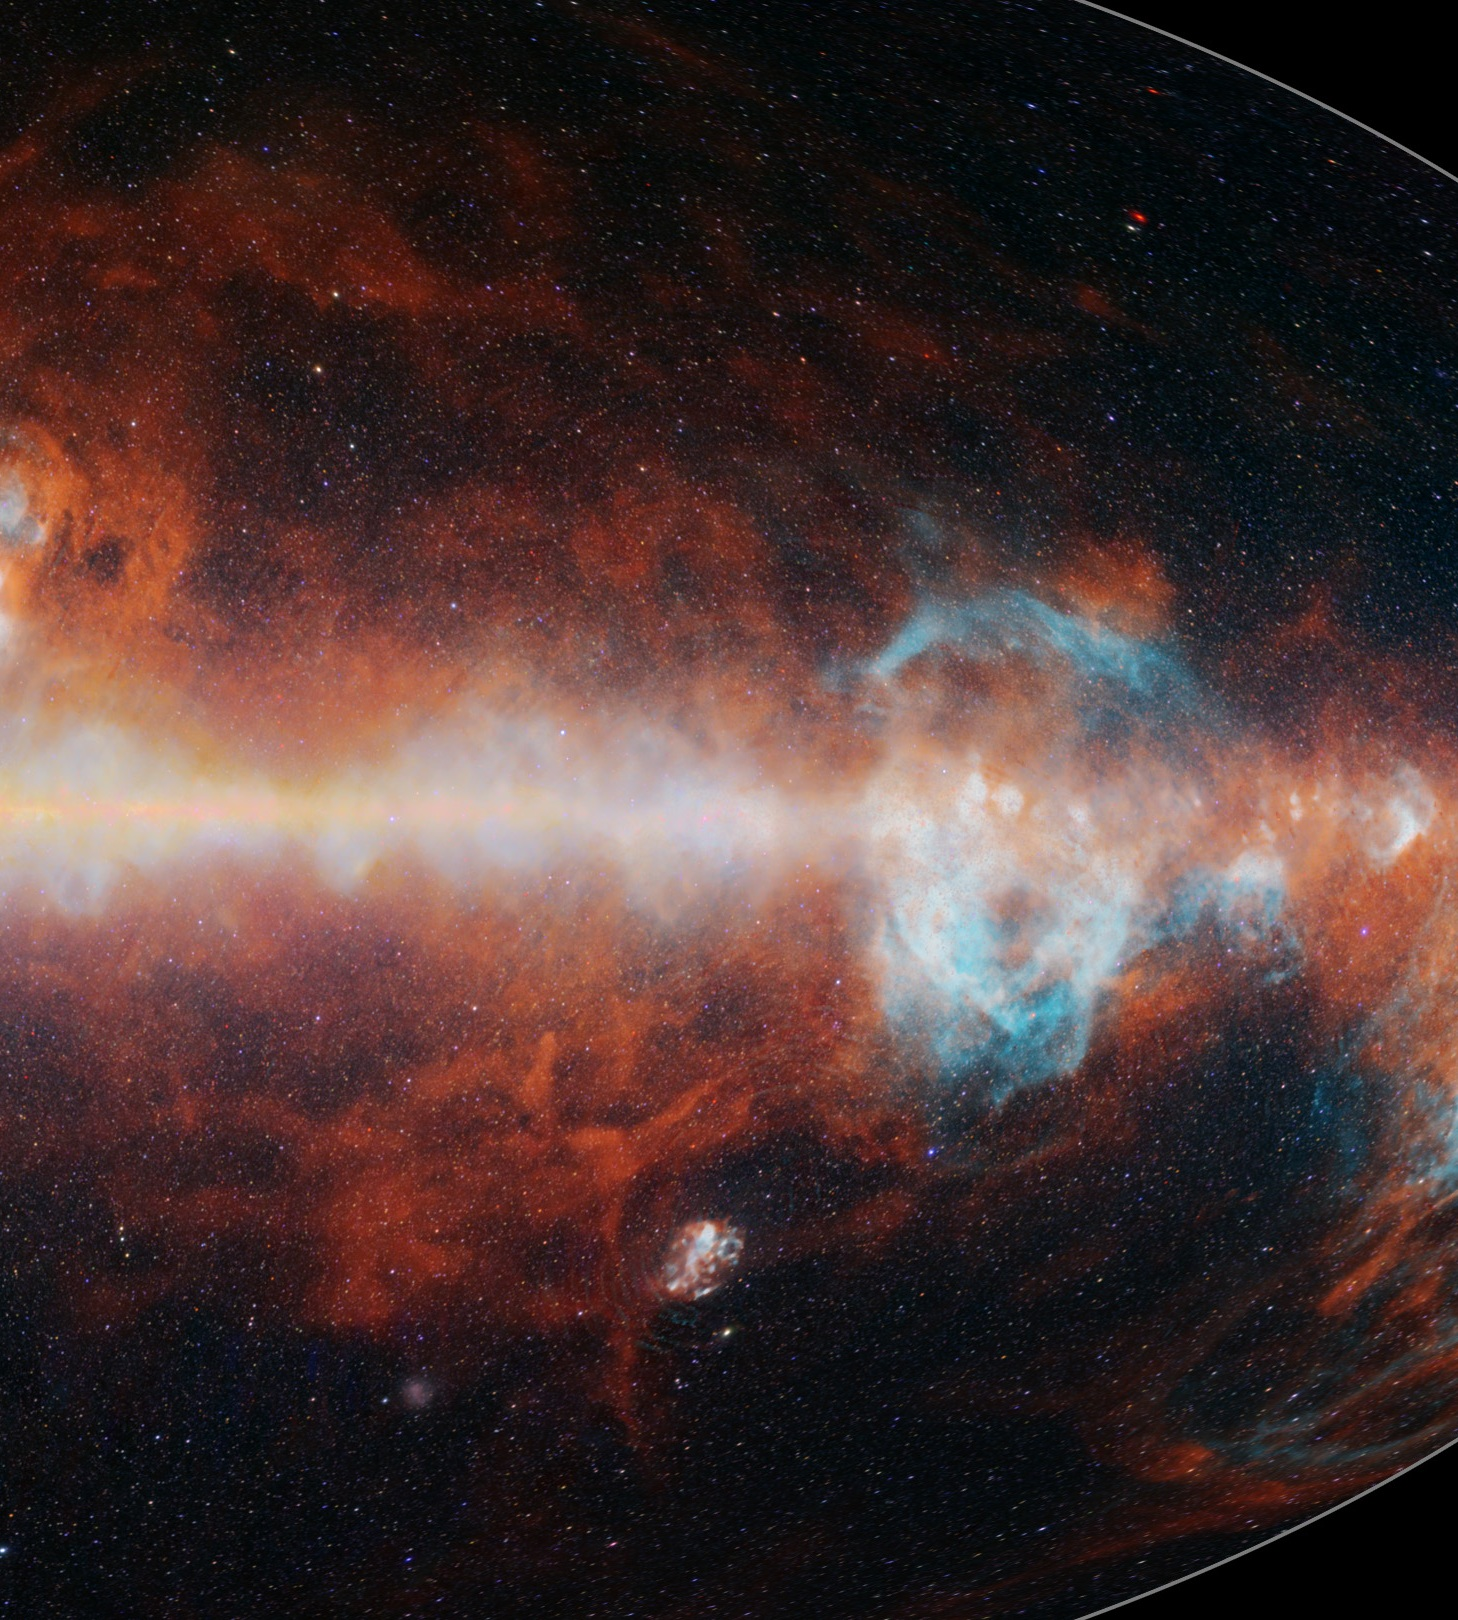
\includegraphics[width=81mm,height=90mm]{spherex-cover.jpg}}
  \fill[Midnight] (0,0) rectangle (79,90);
  \draw[Cyan,line width=.6pt] (79,0) -- (79,90);
  \fill[Midnight] (79.15,0) rectangle (160,8.2);
  \draw[hairline] (79.15,8.2) -- (160,8.2);
  \Place{83}{5.7}{\Caption{\Link{\CoverSource}{SPHEREx all-sky mosaic (crop)}\enspace / \enspace NASA/JPL-Caltech}}

  \Place{8}{83}{\Label{2026 NASA SPACE APPS CHALLENGE}}
  \Place{8}{78.6}{\Caption{Challenge: Planet X and SPHEREx}}
  \Place{7.55}{73.5}{{\fontsize{39}{41}\selectfont\bfseries Paralla\textcolor{Cyan}{X}}}
  \Place{8}{57.8}{\Subhead{Blink the infrared sky}}
  \draw[Cyan,line width=1pt] (8,52.8) -- (25,52.8);
  \Place{8}{49.4}{\Copy{64}{\Body{The blink comparator that found Pluto in 1930, rebuilt for SPHEREx. Type a star name or RA/Dec and watch what moves.}}}

  % ---- TEAM: edit names and GitHub usernames below ----
  \draw[hairline] (8,33.6) -- (71,33.6);
  \Place{8}{31.2}{\Label{THE PARALLAX TEAM}}
  \Place{8}{26.6}{\Member{Farhan Alam}{Frozen-afk}}
  \Place{42}{26.6}{\Member{Abhishek Shahi}{ABHISHEKSHAHI597}}
  \Place{8}{21.8}{\Member{Daksh Rathi}{dakshrathi-india}}
  \Place{42}{21.8}{\Member{Aryan Sisodiya}{InfinityxR9}}
  \Place{8}{17.0}{\Member{Tanmay Pratap Singh}{dhmaltps}}

\end{SlideCanvas}
\end{frame}

% 02 -- The challenge: why a naive blink fails
\begin{frame}[plain]
\begin{SlideCanvas}
  \Heading{THE CHALLENGE}{A raw blink shows colour, not motion}
  \def\PointW{64}

  \Point{10.5}{66.6}{1}{Each frame sees a new colour}{Blink raw frames and \EpsInd{} flickers: it doubles in brightness from 3.25 to 3.58\um.}
  \Point{10.5}{52.0}{2}{Real motion is tiny}{Barnard's Star, the fastest star in our sky, moves about 10\asec{} a year: under 2 pixels.}
  \Point{10.5}{37.4}{3}{Catalogue positions go stale}{The brief's WISE 0855 coordinate is from 2010. The brown dwarf has moved 2\amin{} since.}

  \Place{8}{22.4}{\Label{OUR ANSWER}}
  \Place{8}{18.6}{\Copy{68}{\SmallBody{Compare like with like: one band, one visit, one grid, one brightness scale.}}}

  \Place{84}{66.6}{\Label{SAME SKY, TWO WAVELENGTHS}}
  \begin{scope}
    \clip (84,62.4) rectangle (118,24.15);
    \Place{84}{62.4}{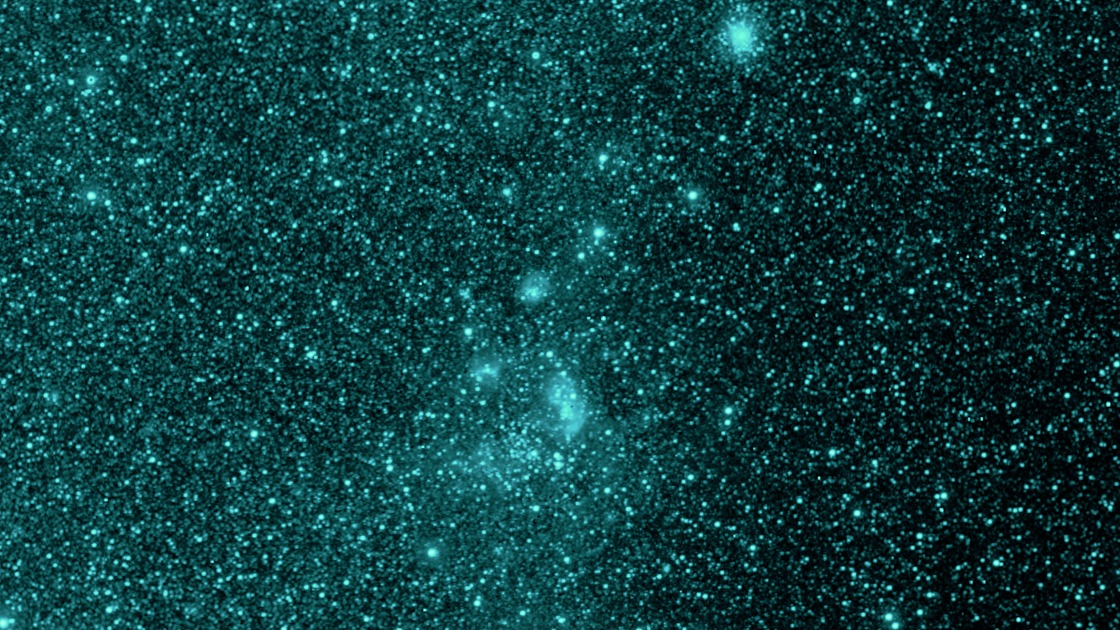
\includegraphics[width=68mm,height=38.25mm]{spherex-vela-098.jpg}}
  \end{scope}
  \begin{scope}
    \clip (118,62.4) rectangle (152,24.15);
    \Place{84}{62.4}{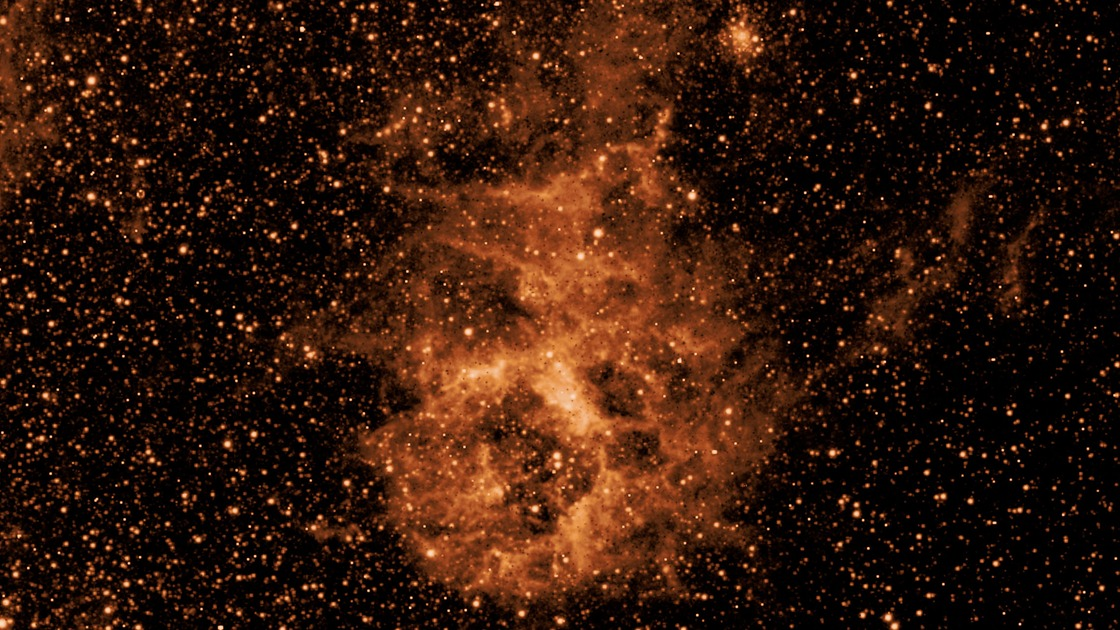
\includegraphics[width=68mm,height=38.25mm]{spherex-vela-329.jpg}}
  \end{scope}
  \draw[hairline] (84,62.4) rectangle (152,24.15);
  \draw[Ink,line width=.6pt] (118,62.4) -- (118,24.15);
  \node[tag] at (85.4,61) {0.98\um};
  \node[tag,anchor=north east] at (150.6,61) {3.29\um};
  \Place{84}{21.9}{\Copy{68}{\Caption{The same Vela field changes with colour alone. False colour, \Link{\VelaSource}{NASA/JPL-Caltech}.}}}
  \Footer{02}
\end{SlideCanvas}
\end{frame}

% 03 -- The solution: how a view is built
\begin{frame}[plain]
\begin{SlideCanvas}
  \Heading{THE SOLUTION}{Stack each visit, then blink}

  \Place{8}{66.6}{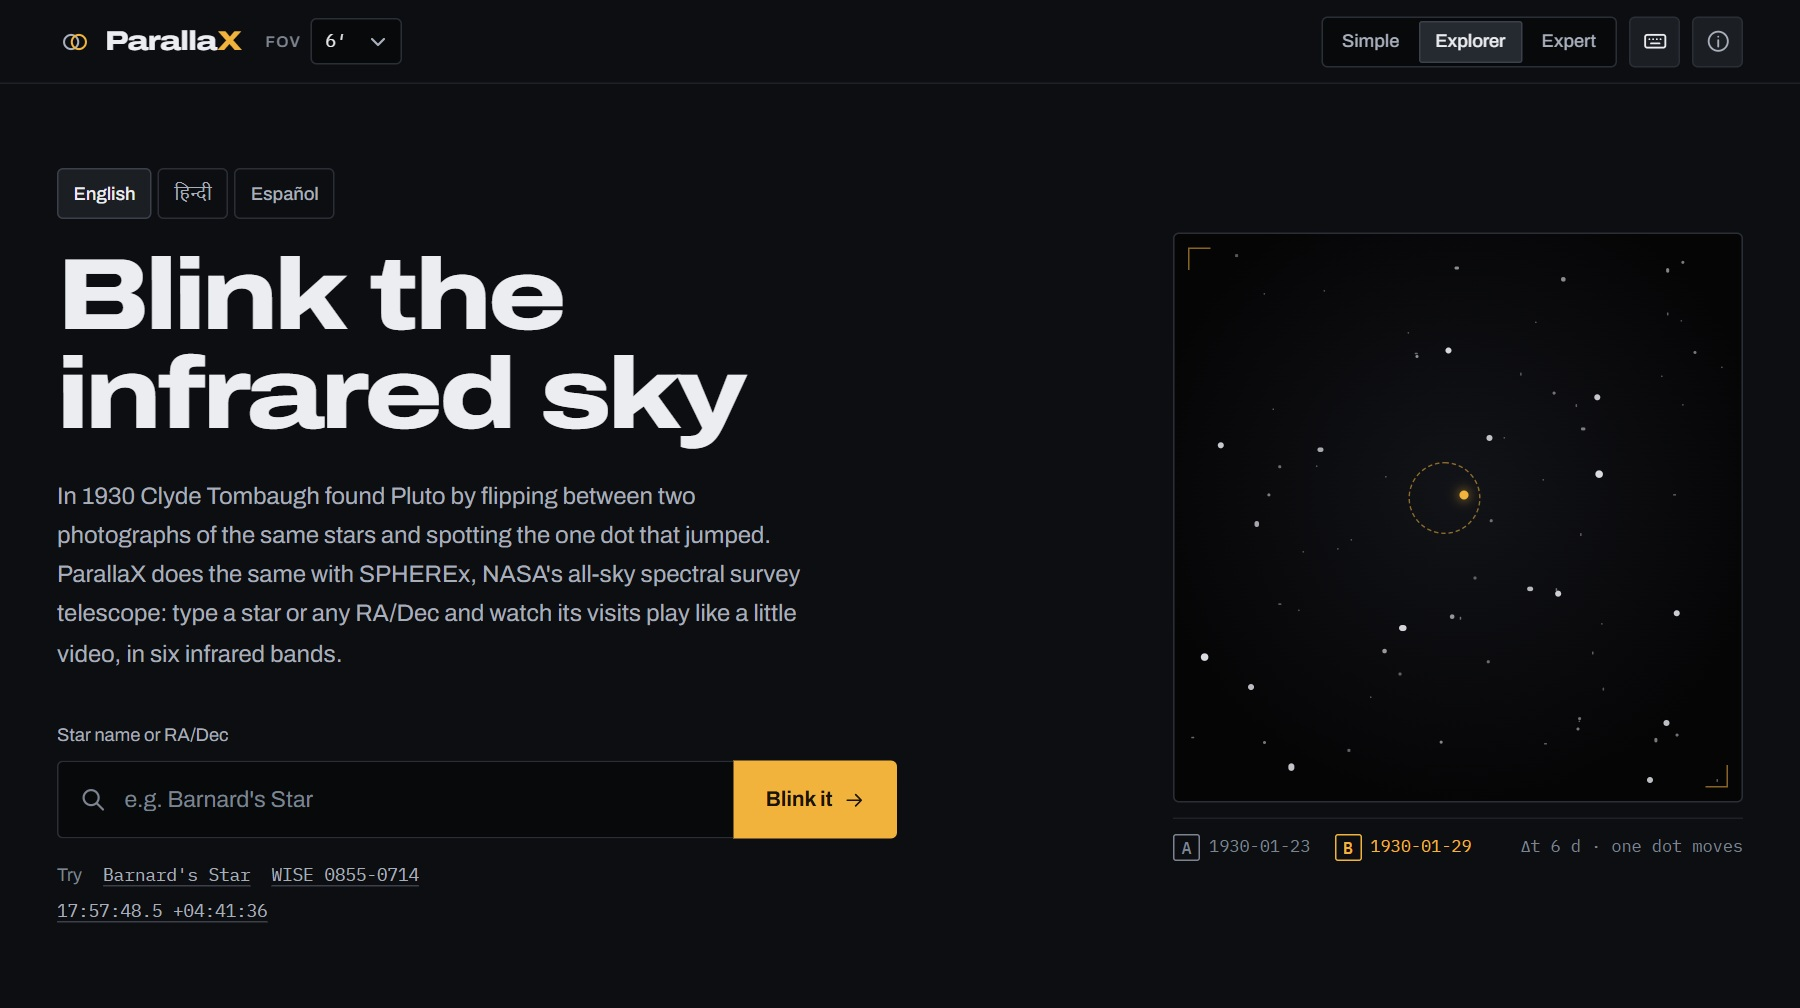
\includegraphics[width=70mm,height=39.2mm]{parallax-home.jpg}}
  \draw[hairline] (8,66.6) rectangle (78,27.4);
  \Place{8}{25.3}{\Caption{The ParallaX home page: search, or open a mission.}}

  \draw[hairline] (86.5,65.1) -- (86.5,35.9);
  \Point{86.5}{66.6}{1}{Find every frame}{SIA2 and TAP, two independent archive routes, must agree. Then split into visits.}
  \Point{86.5}{52.0}{2}{Stack each band}{Mask flagged pixels, remove sky, reproject north-up onto one grid.}
  \Point{86.5}{37.4}{3}{Blink like with like}{One band, one brightness scale for every visit. Play, step, share the link.}

  \path[layer] (8,19.6) rectangle (152,11.6);
  \Place[anchor=base west]{11.2}{14.6}{\Label{BUILT WITH}}
  \Place[anchor=base west]{33}{14.6}{\SmallBody{FastAPI, NumPy, Astropy, reproject \enspace/\enspace React, TypeScript, WebGL2, Aladin Lite}}
  \Footer{03}
\end{SlideCanvas}
\end{frame}

% 04 -- Relevance: the brief, item by item
\begin{frame}[plain]
\begin{SlideCanvas}
  \Heading{RELEVANCE}{Every item in the brief, on NASA data}

  \Place{8}{66.6}{\Label{REQUIRED BY THE BRIEF}}
  \Item{8}{62.0}{Public-facing web tool}{No login; phones; works without WebGL.}
  \Item{8}{53.8}{Enter RA and Dec}{Or a star name. Stale positions are flagged.}
  \Item{8}{45.6}{Images like a little video}{One stack per visit, played as a blink.}
  \Item{8}{37.4}{Easy to spot moving objects}{Track overlay, motion vector, 25-year blink.}
  \Item{8}{29.2}{Test on the five targets}{A one-click mission for each of the five.}

  \Place{80}{66.6}{\Label{OPTIONAL EXTRAS IN THE BRIEF}}
  \Item{80}{62.0}{Easy to update with new data}{Each new data release is one config entry.}
  \Item{80}{53.8}{Show the 102 colours}{Band stacks, RGB, flipbook, spectra.}
  \Item{80}{45.6}{Add or subtract images}{Wavelength-matched difference images.}
  \Item{80}{37.4}{Field of view, link, embedding}{Zoom; the link holds the view; /embed.}
  \Item{80}{29.2}{Gaia and WISE overlays, flags}{Overlays at each visit's epoch; a flag layer.}

  \path[layer] (8,20.8) rectangle (152,10.2);
  \Place{11.2}{18.6}{\Label{NASA DATA AT THE CORE}}
  \Place[anchor=north east]{148.8}{18.6}{\Label{\textcolor{Muted}{PARTNER DATA: ESA GAIA DR3}}}
  \Place{11.2}{14.6}{\SmallBody{SPHEREx QR2 + QR3 (\Link{\Archive}{NASA/IPAC IRSA}) \enspace/\enspace 2MASS \enspace/\enspace AllWISE, NEOWISE \enspace/\enspace JPL Horizons}}
  \Footer{04}
\end{SlideCanvas}
\end{frame}

% 05 -- Creativity: what is new
\begin{frame}[plain]
\begin{SlideCanvas}
  \Heading{WHAT IS NEW}{Built for a spectral imager}

  \Card{8}{66.6}{01}{Visit-stack blink}{One stack per visit and band, so stars hold still and only real change moves.}
  \Card{57.33}{66.6}{02}{25-year blink}{Old 2MASS and WISE frames, then SPHEREx: Barnard's Star jumps 4.5\amin.}
  \Card{106.67}{66.6}{03}{Epoch-aware search}{Recognises an old position of a fast mover and shows where it is now.}
  \Card{8}{40.1}{04}{Spectra on the fly}{Click a source for its spectrum, or flip through the wavelengths.}
  \Card{57.33}{40.1}{05}{Solar System mode}{JPL Horizons tracks Pluto, the original Planet X, as SPHEREx saw it.}
  \Card{106.67}{40.1}{06}{Planet X search}{Links faint one-visit detections along a distant body's parallax drift.}

  \Place{8}{13.9}{\Caption{Layers beyond the core blink are live and marked unvalidated until independent review.}}
  \Footer{05}
\end{SlideCanvas}
\end{frame}

% 06 -- Validity: measured evidence
\begin{frame}[plain]
\begin{SlideCanvas}
  \Heading{EVIDENCE}{Measured, not claimed}

  \Place{8}{66.6}{\Label{BARNARD'S STAR IN PARALLAX}}
  \Place{8}{62.4}{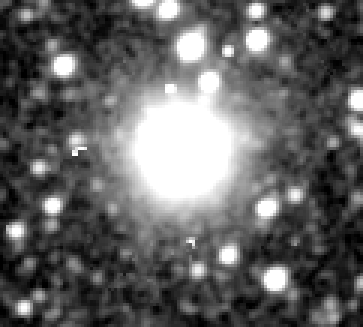
\includegraphics[width=33mm,height=29.73mm]{barnard-v1.png}}
  \Place{44}{62.4}{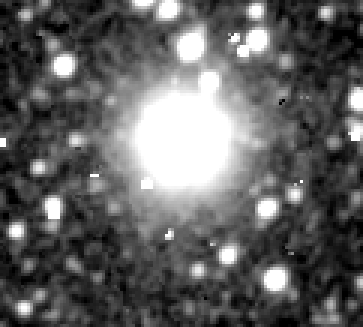
\includegraphics[width=33mm,height=29.73mm]{barnard-v5.png}}
  \draw[hairline] (8,62.4) rectangle (41,32.67);
  \draw[hairline] (44,62.4) rectangle (77,32.67);
  \Place{8}{30.9}{\SmallBody{Visit 1 \enspace Aug 2025}}
  \Place{44}{30.9}{\SmallBody{Visit 5 \enspace Aug 2026}}
  \Place{8}{25.4}{\Caption{Stills from the recorded ParallaX blink}}
  \Place{8}{20.6}{\Copy{69}{\Caption{Development tests passed; independent review pending. Unproven items are published too, such as R Dra's period.}}}

  \Place{84}{66.6}{\Label{MOVED AS PREDICTED (ARCMIN)}}
  \Place{84}{62.4}{\Caption{Target}}
  \Place{109}{62.4}{\Caption{Old survey}}
  \Place[anchor=north east]{139}{62.4}{\Caption{Measured}}
  \Place[anchor=north east]{152}{62.4}{\Caption{Predicted}}
  \foreach \y in {59,53.4,47.8,42.2}{
    \draw[hairline] (84,\y) -- (152,\y);
  }
  \Place{84}{57.4}{\SmallBody{Barnard's Star}}
  \Place{84}{51.8}{\SmallBody{\EpsInd}}
  \Place{84}{46.2}{\SmallBody{WISE 0855$-$0714}}
  \Place{109}{57.4}{\SmallBody{2MASS 2000}}
  \Place{109}{51.8}{\SmallBody{2MASS 1999}}
  \Place{109}{46.2}{\SmallBody{AllWISE 2010}}
  \Place[anchor=north east]{139}{57.4}{\SmallBody{\textcolor{Cyan}{4.540}}}
  \Place[anchor=north east]{139}{51.8}{\SmallBody{\textcolor{Cyan}{2.085}}}
  \Place[anchor=north east]{139}{46.2}{\SmallBody{\textcolor{Cyan}{2.149}}}
  \Place[anchor=north east]{152}{57.4}{\SmallBody{4.540}}
  \Place[anchor=north east]{152}{51.8}{\SmallBody{2.101}}
  \Place[anchor=north east]{152}{46.2}{\SmallBody{2.153}}

  \Stat{38.6}{3,878}{frames for five targets; two archive routes find the same set.}
  \Stat{29.0}{24 / 24}{stacks byte-identical when one link is rebuilt twice from scratch.}
  \Stat{19.4}{0.06\asec/yr}{\EpsInd: motion fitted from SPHEREx alone vs the catalogue.}
  \Footer{06}
\end{SlideCanvas}
\end{frame}

% 07 -- Impact, next steps and links
\begin{frame}[plain]
\begin{SlideCanvas}
  \Heading{WHY IT MATTERS}{Blinking found 3,000 brown dwarfs}

  \Place{8}{66.6}{\Display{\textcolor{Cyan}{3,000+}}}
  \Place{8}{56.4}{\Copy{64}{\Label{BROWN DWARFS FOUND BY VOLUNTEERS BLINKING WISE IMAGES}}}
  \Place{8}{46.6}{\Copy{64}{\Body{WISE has stopped observing. SPHEREx maps the whole sky every six months in 102 colours, and had no public blink tool. Now it has one.}}}
  \Place{8}{26.8}{\Caption{Source: \Link{\BYWSource}{NASA, May 2026 (Backyard Worlds: Planet 9)}}}

  \draw[hairline] (80,24) -- (80,66.6);
  \Place{84}{66.6}{\ItemHead{Citizen scientists}}
  \Place{84}{61.7}{\Copy{68}{\SmallBody{Share any view as a link; open WiseView, ESASky or SIMBAD in a click.}}}
  \Place{84}{52.3}{\ItemHead{Classrooms}}
  \Place{84}{47.4}{\Copy{68}{\SmallBody{A ready 30-minute activity: measure Barnard's Star's motion with a ruler.}}}
  \Place{84}{38.0}{\ItemHead{Everyone}}
  \Place{84}{33.1}{\Copy{68}{\SmallBody{No login, phones, keyboard, a no-WebGL fallback. English, Hindi and Spanish.}}}
  \Footer{07}
\end{SlideCanvas}
\end{frame}

\end{document}
